\section{Experiments}

  In the first experiment, a Gaussian blur was implemented by taking advantage of the
sepearability of the 2D Gaussian function.  To accomplish this all the rows were filtered by a 
1D Gaussian function, then the columns of this image were convolved with the same Gaussian.
This was implemented using a $\sigma$ of 1 and 2.2, the window sizes for these $\sigma$ values
were 5x5 and 11x11 respectively.  The output of this method was compared to the
\texttt{GaussianBlur()} function from OpenCV.

  For the second experiement a Gaussian Pyramid was constructed using two different approaches.
The first approach was to simply convolve the image using a 5x5 gaussian (constructed in the
first experiement), and convolving each new image with the same 5x5 gaussian to construct the
next image.  The other method always used the original image as a base, but changed the size
of the kernel to acheive the same effect.  The $\sigma$ values for the different layers were
defined as $\sigma\sqrt{Layer-1}$ where layer 1 is defined as the original image.

  The third experiement used the Gaussian Pyramid in the second experiement to construct a Laplacian Pyramid.  This was done using a method known as Difference of Gaussians (DoG), which is a close approximation of a laplacian.  The Pyramid was also constructed using the Laplacian opperator, in order to compare the two methods.

  The fourth experiement used the Laplacian Pyramid (constructed using DoG) from experiement three to determine the edge locations in an image.  This was done by locating the zero crossings of the Laplacian at each layer.  The method for locating the zero crossing used here is explained below.

\begin{enumerate}
  \item Threshold the Laplacian using a binary threshold.  The pixels greater than 0 should be given a value of 1, and the negative values should be given a value of 0.
  \item In the thresholded image, set all values which have a neighbor that is a different value than they are to 1 and the others to zero.
  \item Dialate the binary image from step 2.
  \item Find the variance of the pixels in the original Laplacian at locations where the binary image is 1.  All other values in the image should be zero.
  \item Binary threshold the variance image using some user value to obtain edge locations.
  \item Repeat steps 1-5 on all levels of the Laplacian Pyramid.
\end{enumerate}

  The last experiement was to implement edge detection using the Sobel operator.  This can be done by first convolving the original image with the Sobel X and Y operators which yields two images $I_x$ and $I_y$.  The magnitude image is defined as $M(x,y)=|I_x(x,y)| + |I_y(x,y)|$ and the gradient direction is defined as $R(x,y)=atan2(I_y(x,y),I_x(x,y))$.  The edges are obtained by thresholding $M$ using a user defined value.

\section{Results}

%MSE smooth
% lenna 5x5 0.41452
% lenna 11x11 0.450699
% sf 5x5 0.372604
% sf 11x11 0.363327

%MSE gaussian pyramid level
% lenna 1 0
% lenna 2 0
% lenna 3 3.95711
% lenna 4 12.3169
% lenna 5 19.6571
% lenna 6 26.4998
%
% sf 1 0
% sf 2 0
% sf 3 6.6142
% sf 4 13.0404
% sf 5 16.5287
% sf 6 21.4822


\section{Discussion}
\section{Summary}

\newpage

\section{Images}
  %\begin{figure}[hbt]
%  \centering
%  \subfigure[CAP]{
%    \includegraphics[width=0.4\textwidth]{}
%  }
%  \caption{}
%  % Put the label at the bottom
%  \label{fig:}
%\end{figure}

\begin{figure}[hbt]
  \centering
  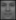
\includegraphics[width=0.25\textwidth]{../results/H_rez/mean_face.jpg}
  \caption{Average face}
  \label{fig:mean}
\end{figure}

~\vfill

\begin{figure}[hbt]
  \centering
  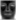
\includegraphics[width=0.18\textwidth]{../results/H_rez/eigenfaces/largest1.jpg}
  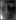
\includegraphics[width=0.18\textwidth]{../results/H_rez/eigenfaces/largest2.jpg}
  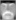
\includegraphics[width=0.18\textwidth]{../results/H_rez/eigenfaces/largest3.jpg}
  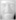
\includegraphics[width=0.18\textwidth]{../results/H_rez/eigenfaces/largest4.jpg}
  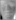
\includegraphics[width=0.18\textwidth]{../results/H_rez/eigenfaces/largest5.jpg} \\
  \vspace{4pt}
  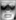
\includegraphics[width=0.18\textwidth]{../results/H_rez/eigenfaces/largest6.jpg}
  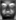
\includegraphics[width=0.18\textwidth]{../results/H_rez/eigenfaces/largest7.jpg}
  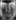
\includegraphics[width=0.18\textwidth]{../results/H_rez/eigenfaces/largest8.jpg}
  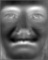
\includegraphics[width=0.18\textwidth]{../results/H_rez/eigenfaces/largest9.jpg}
  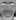
\includegraphics[width=0.18\textwidth]{../results/H_rez/eigenfaces/largest10.jpg}
  \caption{Top ten Eigenfaces}
  \label{fig:top_efaces}
\end{figure}

~\vfill

\begin{figure}[hbt]
  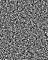
\includegraphics[width=0.09\textwidth]{../results/H_rez/eigenfaces/smallest1.jpg}
  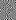
\includegraphics[width=0.09\textwidth]{../results/H_rez/eigenfaces/smallest2.jpg}
  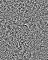
\includegraphics[width=0.09\textwidth]{../results/H_rez/eigenfaces/smallest3.jpg}
  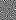
\includegraphics[width=0.09\textwidth]{../results/H_rez/eigenfaces/smallest4.jpg}
  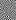
\includegraphics[width=0.09\textwidth]{../results/H_rez/eigenfaces/smallest5.jpg}
  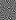
\includegraphics[width=0.09\textwidth]{../results/H_rez/eigenfaces/smallest6.jpg}
  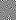
\includegraphics[width=0.09\textwidth]{../results/H_rez/eigenfaces/smallest7.jpg}
  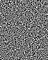
\includegraphics[width=0.09\textwidth]{../results/H_rez/eigenfaces/smallest8.jpg}
  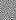
\includegraphics[width=0.09\textwidth]{../results/H_rez/eigenfaces/smallest9.jpg}
  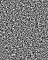
\includegraphics[width=0.09\textwidth]{../results/H_rez/eigenfaces/smallest10.jpg}
  \caption{Bottom ten Eigenfaces}
  \label{fig:bot_efaces}
\end{figure}

~\vfill

\vfill

~\vfill

\begin{figure}[hbt]
  \centering
  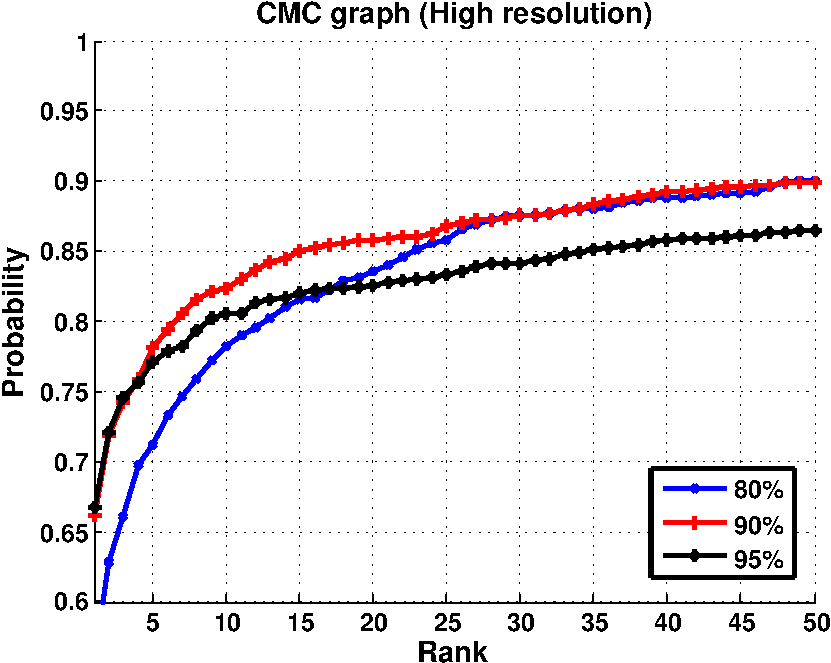
\includegraphics[width=0.7\textwidth]{../results/Output_H.pdf}
  \caption{High resolution CMC for training at 80\%, 90\%, and 95\% information retention.}
  \label{fig:cfc_h}
\end{figure}

~\vfill

\begin{figure}[hbt]
  \centering
  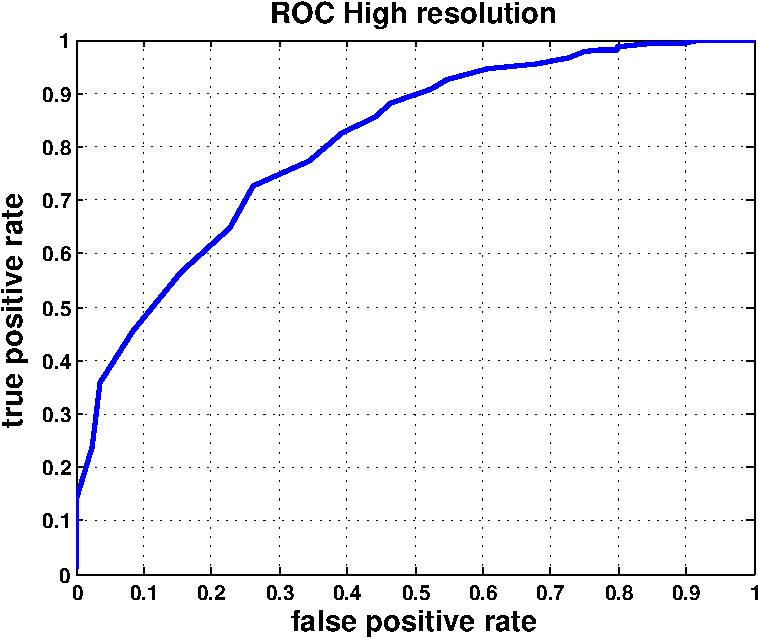
\includegraphics[width=0.7\textwidth]{../results/ROC_H.pdf}
  \caption{High resolution ROC.}
  \label{fig:roc_h}
\end{figure}

~\vfill

\vfill

~\vfill

\begin{figure}[hbt]
  \centering
  \includegraphics[width=0.1\textwidth]{../results/H_rez/correct80/1/testImg.jpg} \vline
  \hspace{2pt}
  \includegraphics[width=42pt]{../results/H_rez/correct80/1/1.jpg}
  \includegraphics[width=42pt]{../results/H_rez/correct80/1/2.jpg}
  \includegraphics[width=31pt]{../results/H_rez/correct80/1/3.jpg}
  \includegraphics[width=42pt]{../results/H_rez/correct80/1/4.jpg}
  \includegraphics[width=31pt]{../results/H_rez/correct80/1/5.jpg}
  \includegraphics[width=31pt]{../results/H_rez/correct80/1/6.jpg}
  \includegraphics[width=42pt]{../results/H_rez/correct80/1/7.jpg}
  \includegraphics[width=42pt]{../results/H_rez/correct80/1/8.jpg}
  \includegraphics[width=31pt]{../results/H_rez/correct80/1/9.jpg}
  \includegraphics[width=31pt]{../results/H_rez/correct80/1/10.jpg} \\
  \vspace{4pt}
  \includegraphics[width=0.1\textwidth]{../results/H_rez/correct80/2/testImg.jpg} \vline
  \hspace{2pt}
  \includegraphics[width=0.09\textwidth]{../results/H_rez/correct80/2/1.jpg}
  \includegraphics[width=0.09\textwidth]{../results/H_rez/correct80/2/2.jpg}
  \includegraphics[width=0.07\textwidth]{../results/H_rez/correct80/2/3.jpg}
  \includegraphics[width=0.09\textwidth]{../results/H_rez/correct80/2/4.jpg}
  \includegraphics[width=0.07\textwidth]{../results/H_rez/correct80/2/5.jpg}
  \includegraphics[width=0.09\textwidth]{../results/H_rez/correct80/2/6.jpg}
  \includegraphics[width=0.07\textwidth]{../results/H_rez/correct80/2/7.jpg}
  \includegraphics[width=0.07\textwidth]{../results/H_rez/correct80/2/8.jpg}
  \includegraphics[width=0.07\textwidth]{../results/H_rez/correct80/2/9.jpg}
  \includegraphics[width=0.07\textwidth]{../results/H_rez/correct80/2/10.jpg} \\
  \vspace{4pt}
  \includegraphics[width=0.1\textwidth]{../results/H_rez/correct80/3/testImg.jpg} \vline
  \hspace{2pt}
  \includegraphics[width=0.09\textwidth]{../results/H_rez/correct80/3/1.jpg}
  \includegraphics[width=0.07\textwidth]{../results/H_rez/correct80/3/2.jpg}
  \includegraphics[width=0.09\textwidth]{../results/H_rez/correct80/3/3.jpg}
  \includegraphics[width=0.07\textwidth]{../results/H_rez/correct80/3/4.jpg}
  \includegraphics[width=0.09\textwidth]{../results/H_rez/correct80/3/5.jpg}
  \includegraphics[width=0.07\textwidth]{../results/H_rez/correct80/3/6.jpg}
  \includegraphics[width=0.07\textwidth]{../results/H_rez/correct80/3/7.jpg}
  \includegraphics[width=0.07\textwidth]{../results/H_rez/correct80/3/8.jpg}
  \includegraphics[width=0.07\textwidth]{../results/H_rez/correct80/3/9.jpg}
  \includegraphics[width=0.09\textwidth]{../results/H_rez/correct80/3/10.jpg}
  \caption{Top matches for 3 correctly matched faces at 80\% information retention.}
  \label{fig:correct80}
\end{figure}

~\vfill

\begin{figure}[hbt]
  \centering
  \includegraphics[width=0.1\textwidth]{../results/H_rez/incorrect80/1/testImg.jpg} \vline
  \hspace{2pt}
  \includegraphics[width=0.08\textwidth]{../results/H_rez/incorrect80/1/1.jpg}
  \includegraphics[width=0.08\textwidth]{../results/H_rez/incorrect80/1/2.jpg}
  \includegraphics[width=0.08\textwidth]{../results/H_rez/incorrect80/1/3.jpg}
  \includegraphics[width=0.08\textwidth]{../results/H_rez/incorrect80/1/4.jpg}
  \includegraphics[width=0.08\textwidth]{../results/H_rez/incorrect80/1/5.jpg}
  \includegraphics[width=0.08\textwidth]{../results/H_rez/incorrect80/1/6.jpg}
  \includegraphics[width=0.08\textwidth]{../results/H_rez/incorrect80/1/7.jpg}
  \includegraphics[width=0.08\textwidth]{../results/H_rez/incorrect80/1/8.jpg}
  \includegraphics[width=0.08\textwidth]{../results/H_rez/incorrect80/1/9.jpg}
  \includegraphics[width=0.08\textwidth]{../results/H_rez/incorrect80/1/10.jpg} \\
  \vspace{4pt}
  \includegraphics[width=0.1\textwidth]{../results/H_rez/incorrect80/2/testImg.jpg} \vline
  \hspace{2pt}
  \includegraphics[width=0.08\textwidth]{../results/H_rez/incorrect80/2/1.jpg}
  \includegraphics[width=0.08\textwidth]{../results/H_rez/incorrect80/2/2.jpg}
  \includegraphics[width=0.08\textwidth]{../results/H_rez/incorrect80/2/3.jpg}
  \includegraphics[width=0.08\textwidth]{../results/H_rez/incorrect80/2/4.jpg}
  \includegraphics[width=0.08\textwidth]{../results/H_rez/incorrect80/2/5.jpg}
  \includegraphics[width=0.08\textwidth]{../results/H_rez/incorrect80/2/6.jpg}
  \includegraphics[width=0.08\textwidth]{../results/H_rez/incorrect80/2/7.jpg}
  \includegraphics[width=0.08\textwidth]{../results/H_rez/incorrect80/2/8.jpg}
  \includegraphics[width=0.08\textwidth]{../results/H_rez/incorrect80/2/8.jpg}
  \includegraphics[width=0.08\textwidth]{../results/H_rez/incorrect80/2/10.jpg} \\
  \vspace{4pt}
  \includegraphics[width=0.1\textwidth]{../results/H_rez/incorrect80/3/testImg.jpg} \vline
  \hspace{2pt}
  \includegraphics[width=0.08\textwidth]{../results/H_rez/incorrect80/3/1.jpg}
  \includegraphics[width=0.08\textwidth]{../results/H_rez/incorrect80/3/2.jpg}
  \includegraphics[width=0.08\textwidth]{../results/H_rez/incorrect80/3/3.jpg}
  \includegraphics[width=0.08\textwidth]{../results/H_rez/incorrect80/3/4.jpg}
  \includegraphics[width=0.08\textwidth]{../results/H_rez/incorrect80/3/5.jpg}
  \includegraphics[width=0.08\textwidth]{../results/H_rez/incorrect80/3/6.jpg}
  \includegraphics[width=0.08\textwidth]{../results/H_rez/incorrect80/3/7.jpg}
  \includegraphics[width=0.08\textwidth]{../results/H_rez/incorrect80/3/8.jpg}
  \includegraphics[width=0.08\textwidth]{../results/H_rez/incorrect80/3/8.jpg}
  \includegraphics[width=0.08\textwidth]{../results/H_rez/incorrect80/3/10.jpg}
  \caption{Top matches for 3 incorrectly matched faces at 80\% information retention.}
  \label{fig:incorrect80}
\end{figure}

~\vfill

\clearpage

~\vfill

\begin{figure}[hbt]
  \centering
  \includegraphics[width=0.1\textwidth]{../results/H_rez/correct90/1/testImg.jpg} \vline
  \hspace{2pt}
  \includegraphics[width=0.09\textwidth]{../results/H_rez/correct90/1/1.jpg}
  \includegraphics[width=0.09\textwidth]{../results/H_rez/correct90/1/2.jpg}
  \includegraphics[width=0.09\textwidth]{../results/H_rez/correct90/1/3.jpg}
  \includegraphics[width=0.09\textwidth]{../results/H_rez/correct90/1/4.jpg}
  \includegraphics[width=0.06\textwidth]{../results/H_rez/correct90/1/5.jpg}
  \includegraphics[width=0.09\textwidth]{../results/H_rez/correct90/1/6.jpg}
  \includegraphics[width=0.06\textwidth]{../results/H_rez/correct90/1/7.jpg}
  \includegraphics[width=0.09\textwidth]{../results/H_rez/correct90/1/8.jpg}
  \includegraphics[width=0.06\textwidth]{../results/H_rez/correct90/1/9.jpg}
  \includegraphics[width=0.06\textwidth]{../results/H_rez/correct90/1/10.jpg} \\
  \vspace{4pt}
  \includegraphics[width=0.1\textwidth]{../results/H_rez/correct90/2/testImg.jpg} \vline
  \hspace{2pt}
  \includegraphics[width=0.09\textwidth]{../results/H_rez/correct90/2/1.jpg}
  \includegraphics[width=0.09\textwidth]{../results/H_rez/correct90/2/2.jpg}
  \includegraphics[width=0.09\textwidth]{../results/H_rez/correct90/2/3.jpg}
  \includegraphics[width=0.09\textwidth]{../results/H_rez/correct90/2/4.jpg}
  \includegraphics[width=0.09\textwidth]{../results/H_rez/correct90/2/5.jpg}
  \includegraphics[width=0.09\textwidth]{../results/H_rez/correct90/2/6.jpg}
  \includegraphics[width=0.06\textwidth]{../results/H_rez/correct90/2/7.jpg}
  \includegraphics[width=0.06\textwidth]{../results/H_rez/correct90/2/8.jpg}
  \includegraphics[width=0.06\textwidth]{../results/H_rez/correct90/2/8.jpg}
  \includegraphics[width=0.06\textwidth]{../results/H_rez/correct90/2/10.jpg} \\
  \vspace{4pt}
  \includegraphics[width=0.1\textwidth]{../results/H_rez/correct90/3/testImg.jpg} \vline
  \hspace{2pt}
  \includegraphics[width=0.09\textwidth]{../results/H_rez/correct90/3/1.jpg}
  \includegraphics[width=0.09\textwidth]{../results/H_rez/correct90/3/2.jpg}
  \includegraphics[width=0.09\textwidth]{../results/H_rez/correct90/3/3.jpg}
  \includegraphics[width=0.07\textwidth]{../results/H_rez/correct90/3/4.jpg}
  \includegraphics[width=0.07\textwidth]{../results/H_rez/correct90/3/5.jpg}
  \includegraphics[width=0.07\textwidth]{../results/H_rez/correct90/3/6.jpg}
  \includegraphics[width=0.07\textwidth]{../results/H_rez/correct90/3/7.jpg}
  \includegraphics[width=0.07\textwidth]{../results/H_rez/correct90/3/8.jpg}
  \includegraphics[width=0.07\textwidth]{../results/H_rez/correct90/3/8.jpg}
  \includegraphics[width=0.09\textwidth]{../results/H_rez/correct90/3/10.jpg}
  \caption{Top matches for 3 correctly matched faces at 90\% information retention.}
  \label{fig:correct90}
\end{figure}

~\vfill

\begin{figure}[hbt]
  \centering
  \includegraphics[width=0.1\textwidth]{../results/H_rez/incorrect90/1/testImg.jpg} \vline
  \hspace{2pt}
  \includegraphics[width=0.08\textwidth]{../results/H_rez/incorrect90/1/1.jpg}
  \includegraphics[width=0.08\textwidth]{../results/H_rez/incorrect90/1/2.jpg}
  \includegraphics[width=0.08\textwidth]{../results/H_rez/incorrect90/1/3.jpg}
  \includegraphics[width=0.08\textwidth]{../results/H_rez/incorrect90/1/4.jpg}
  \includegraphics[width=0.08\textwidth]{../results/H_rez/incorrect90/1/5.jpg}
  \includegraphics[width=0.08\textwidth]{../results/H_rez/incorrect90/1/6.jpg}
  \includegraphics[width=0.08\textwidth]{../results/H_rez/incorrect90/1/7.jpg}
  \includegraphics[width=0.08\textwidth]{../results/H_rez/incorrect90/1/8.jpg}
  \includegraphics[width=0.08\textwidth]{../results/H_rez/incorrect90/1/9.jpg}
  \includegraphics[width=0.08\textwidth]{../results/H_rez/incorrect90/1/10.jpg} \\
  \vspace{4pt}
  \includegraphics[width=0.1\textwidth]{../results/H_rez/incorrect90/2/testImg.jpg} \vline
  \hspace{2pt}
  \includegraphics[width=0.08\textwidth]{../results/H_rez/incorrect90/2/1.jpg}
  \includegraphics[width=0.08\textwidth]{../results/H_rez/incorrect90/2/2.jpg}
  \includegraphics[width=0.08\textwidth]{../results/H_rez/incorrect90/2/3.jpg}
  \includegraphics[width=0.08\textwidth]{../results/H_rez/incorrect90/2/4.jpg}
  \includegraphics[width=0.08\textwidth]{../results/H_rez/incorrect90/2/5.jpg}
  \includegraphics[width=0.08\textwidth]{../results/H_rez/incorrect90/2/6.jpg}
  \includegraphics[width=0.08\textwidth]{../results/H_rez/incorrect90/2/7.jpg}
  \includegraphics[width=0.08\textwidth]{../results/H_rez/incorrect90/2/8.jpg}
  \includegraphics[width=0.08\textwidth]{../results/H_rez/incorrect90/2/8.jpg}
  \includegraphics[width=0.08\textwidth]{../results/H_rez/incorrect90/2/10.jpg} \\
  \vspace{4pt}
  \includegraphics[width=0.1\textwidth]{../results/H_rez/incorrect90/3/testImg.jpg} \vline
  \hspace{2pt}
  \includegraphics[width=0.08\textwidth]{../results/H_rez/incorrect90/3/1.jpg}
  \includegraphics[width=0.08\textwidth]{../results/H_rez/incorrect90/3/2.jpg}
  \includegraphics[width=0.08\textwidth]{../results/H_rez/incorrect90/3/3.jpg}
  \includegraphics[width=0.08\textwidth]{../results/H_rez/incorrect90/3/4.jpg}
  \includegraphics[width=0.08\textwidth]{../results/H_rez/incorrect90/3/5.jpg}
  \includegraphics[width=0.08\textwidth]{../results/H_rez/incorrect90/3/6.jpg}
  \includegraphics[width=0.08\textwidth]{../results/H_rez/incorrect90/3/7.jpg}
  \includegraphics[width=0.08\textwidth]{../results/H_rez/incorrect90/3/8.jpg}
  \includegraphics[width=0.08\textwidth]{../results/H_rez/incorrect90/3/8.jpg}
  \includegraphics[width=0.08\textwidth]{../results/H_rez/incorrect90/3/10.jpg}
  \caption{Top matches for 3 incorrectly matched faces at 90\% information retention.}
  \label{fig:incorrect90}
\end{figure}

~\vfill

\clearpage

~\vfill

\begin{figure}[hbt]
  \centering
  \includegraphics[width=0.1\textwidth]{../results/H_rez/correct95/1/testImg.jpg} \vline
  \hspace{2pt}
  \includegraphics[width=0.09\textwidth]{../results/H_rez/correct95/1/1.jpg}
  \includegraphics[width=0.09\textwidth]{../results/H_rez/correct95/1/2.jpg}
  \includegraphics[width=0.09\textwidth]{../results/H_rez/correct95/1/3.jpg}
  \includegraphics[width=0.09\textwidth]{../results/H_rez/correct95/1/4.jpg}
  \includegraphics[width=0.06\textwidth]{../results/H_rez/correct95/1/5.jpg}
  \includegraphics[width=0.09\textwidth]{../results/H_rez/correct95/1/6.jpg}
  \includegraphics[width=0.06\textwidth]{../results/H_rez/correct95/1/7.jpg}
  \includegraphics[width=0.06\textwidth]{../results/H_rez/correct95/1/8.jpg}
  \includegraphics[width=0.09\textwidth]{../results/H_rez/correct95/1/9.jpg}
  \includegraphics[width=0.06\textwidth]{../results/H_rez/correct95/1/10.jpg} \\
  \vspace{4pt}
  \includegraphics[width=0.1\textwidth]{../results/H_rez/correct95/2/testImg.jpg} \vline
  \hspace{2pt}
  \includegraphics[width=0.09\textwidth]{../results/H_rez/correct95/2/1.jpg}
  \includegraphics[width=0.09\textwidth]{../results/H_rez/correct95/2/2.jpg}
  \includegraphics[width=0.07\textwidth]{../results/H_rez/correct95/2/3.jpg}
  \includegraphics[width=0.07\textwidth]{../results/H_rez/correct95/2/4.jpg}
  \includegraphics[width=0.09\textwidth]{../results/H_rez/correct95/2/5.jpg}
  \includegraphics[width=0.07\textwidth]{../results/H_rez/correct95/2/6.jpg}
  \includegraphics[width=0.09\textwidth]{../results/H_rez/correct95/2/7.jpg}
  \includegraphics[width=0.07\textwidth]{../results/H_rez/correct95/2/8.jpg}
  \includegraphics[width=0.07\textwidth]{../results/H_rez/correct95/2/8.jpg}
  \includegraphics[width=0.07\textwidth]{../results/H_rez/correct95/2/10.jpg} \\
  \vspace{4pt}
  \includegraphics[width=0.1\textwidth]{../results/H_rez/correct95/3/testImg.jpg} \vline
  \hspace{2pt}
  \includegraphics[width=0.09\textwidth]{../results/H_rez/correct95/3/1.jpg}
  \includegraphics[width=0.09\textwidth]{../results/H_rez/correct95/3/2.jpg}
  \includegraphics[width=0.09\textwidth]{../results/H_rez/correct95/3/3.jpg}
  \includegraphics[width=0.07\textwidth]{../results/H_rez/correct95/3/4.jpg}
  \includegraphics[width=0.09\textwidth]{../results/H_rez/correct95/3/5.jpg}
  \includegraphics[width=0.07\textwidth]{../results/H_rez/correct95/3/6.jpg}
  \includegraphics[width=0.07\textwidth]{../results/H_rez/correct95/3/7.jpg}
  \includegraphics[width=0.07\textwidth]{../results/H_rez/correct95/3/8.jpg}
  \includegraphics[width=0.07\textwidth]{../results/H_rez/correct95/3/8.jpg}
  \includegraphics[width=0.07\textwidth]{../results/H_rez/correct95/3/10.jpg}
  \caption{Top matches for 3 correctly matched faces at 95\% information retention.}
  \label{fig:correct95}
\end{figure}

~\vfill

\begin{figure}[hbt]
  \centering
  \includegraphics[width=0.1\textwidth]{../results/H_rez/incorrect95/1/testImg.jpg} \vline
  \hspace{2pt}
  \includegraphics[width=0.08\textwidth]{../results/H_rez/incorrect95/1/1.jpg}
  \includegraphics[width=0.08\textwidth]{../results/H_rez/incorrect95/1/2.jpg}
  \includegraphics[width=0.08\textwidth]{../results/H_rez/incorrect95/1/3.jpg}
  \includegraphics[width=0.08\textwidth]{../results/H_rez/incorrect95/1/4.jpg}
  \includegraphics[width=0.08\textwidth]{../results/H_rez/incorrect95/1/5.jpg}
  \includegraphics[width=0.08\textwidth]{../results/H_rez/incorrect95/1/6.jpg}
  \includegraphics[width=0.08\textwidth]{../results/H_rez/incorrect95/1/7.jpg}
  \includegraphics[width=0.08\textwidth]{../results/H_rez/incorrect95/1/8.jpg}
  \includegraphics[width=0.08\textwidth]{../results/H_rez/incorrect95/1/9.jpg}
  \includegraphics[width=0.08\textwidth]{../results/H_rez/incorrect95/1/10.jpg} \\
  \vspace{4pt}
  \includegraphics[width=0.1\textwidth]{../results/H_rez/incorrect95/2/testImg.jpg} \vline
  \hspace{2pt}
  \includegraphics[width=0.08\textwidth]{../results/H_rez/incorrect95/2/1.jpg}
  \includegraphics[width=0.08\textwidth]{../results/H_rez/incorrect95/2/2.jpg}
  \includegraphics[width=0.08\textwidth]{../results/H_rez/incorrect95/2/3.jpg}
  \includegraphics[width=0.08\textwidth]{../results/H_rez/incorrect95/2/4.jpg}
  \includegraphics[width=0.08\textwidth]{../results/H_rez/incorrect95/2/5.jpg}
  \includegraphics[width=0.08\textwidth]{../results/H_rez/incorrect95/2/6.jpg}
  \includegraphics[width=0.08\textwidth]{../results/H_rez/incorrect95/2/7.jpg}
  \includegraphics[width=0.08\textwidth]{../results/H_rez/incorrect95/2/8.jpg}
  \includegraphics[width=0.08\textwidth]{../results/H_rez/incorrect95/2/8.jpg}
  \includegraphics[width=0.08\textwidth]{../results/H_rez/incorrect95/2/10.jpg} \\
  \vspace{4pt}
  \includegraphics[width=0.1\textwidth]{../results/H_rez/incorrect95/3/testImg.jpg} \vline
  \hspace{2pt}
  \includegraphics[width=0.08\textwidth]{../results/H_rez/incorrect95/3/1.jpg}
  \includegraphics[width=0.08\textwidth]{../results/H_rez/incorrect95/3/2.jpg}
  \includegraphics[width=0.08\textwidth]{../results/H_rez/incorrect95/3/3.jpg}
  \includegraphics[width=0.08\textwidth]{../results/H_rez/incorrect95/3/4.jpg}
  \includegraphics[width=0.08\textwidth]{../results/H_rez/incorrect95/3/5.jpg}
  \includegraphics[width=0.08\textwidth]{../results/H_rez/incorrect95/3/6.jpg}
  \includegraphics[width=0.08\textwidth]{../results/H_rez/incorrect95/3/7.jpg}
  \includegraphics[width=0.08\textwidth]{../results/H_rez/incorrect95/3/8.jpg}
  \includegraphics[width=0.08\textwidth]{../results/H_rez/incorrect95/3/8.jpg}
  \includegraphics[width=0.08\textwidth]{../results/H_rez/incorrect95/3/10.jpg}
  \caption{Top matches for 3 incorrectly matched faces at 95\% information retention.}
  \label{fig:incorrect95}
\end{figure}

~\vfill

\clearpage

~\vfill

\begin{figure}[hbt]
  \centering
  \includegraphics[width=0.25\textwidth]{../results/L_rez/mean_face.jpg}
  \caption{Average face (Low res)}
  \label{fig:mean_l}
\end{figure}

~\vfill

\begin{figure}[hbt]
  \centering
  \includegraphics[width=0.18\textwidth]{../results/L_rez/eigenfaces/largest1.jpg}
  \includegraphics[width=0.18\textwidth]{../results/L_rez/eigenfaces/largest2.jpg}
  \includegraphics[width=0.18\textwidth]{../results/L_rez/eigenfaces/largest3.jpg}
  \includegraphics[width=0.18\textwidth]{../results/L_rez/eigenfaces/largest4.jpg}
  \includegraphics[width=0.18\textwidth]{../results/L_rez/eigenfaces/largest5.jpg} \\
  \vspace{4pt}
  \includegraphics[width=0.18\textwidth]{../results/L_rez/eigenfaces/largest6.jpg}
  \includegraphics[width=0.18\textwidth]{../results/L_rez/eigenfaces/largest7.jpg}
  \includegraphics[width=0.18\textwidth]{../results/L_rez/eigenfaces/largest8.jpg}
  \includegraphics[width=0.18\textwidth]{../results/L_rez/eigenfaces/largest9.jpg}
  \includegraphics[width=0.18\textwidth]{../results/L_rez/eigenfaces/largest10.jpg}
  \caption{Top ten low resolution Eigenfaces}
  \label{fig:top_efaces_l}
\end{figure}

~\vfill

\begin{figure}[hbt]
  \includegraphics[width=0.09\textwidth]{../results/L_rez/eigenfaces/smallest1.jpg}
  \includegraphics[width=0.09\textwidth]{../results/L_rez/eigenfaces/smallest2.jpg}
  \includegraphics[width=0.09\textwidth]{../results/L_rez/eigenfaces/smallest3.jpg}
  \includegraphics[width=0.09\textwidth]{../results/L_rez/eigenfaces/smallest4.jpg}
  \includegraphics[width=0.09\textwidth]{../results/L_rez/eigenfaces/smallest5.jpg}
  \includegraphics[width=0.09\textwidth]{../results/L_rez/eigenfaces/smallest6.jpg}
  \includegraphics[width=0.09\textwidth]{../results/L_rez/eigenfaces/smallest7.jpg}
  \includegraphics[width=0.09\textwidth]{../results/L_rez/eigenfaces/smallest8.jpg}
  \includegraphics[width=0.09\textwidth]{../results/L_rez/eigenfaces/smallest9.jpg}
  \includegraphics[width=0.09\textwidth]{../results/L_rez/eigenfaces/smallest10.jpg}
  \caption{Bottom ten low resolution Eigenfaces}
  \label{fig:bot_efaces_l}
\end{figure}

~\vfill

\vfill

~\vfill

\begin{figure}[hbt]
  \centering
  \includegraphics[width=0.7\textwidth]{../results/Output_L.pdf}
  \caption{Low resolution CMC for training at 80\%, 90\%, and 95\% information retention.}
  \label{fig:cfc_l}
\end{figure}

\begin{figure}[hbt]
  \centering
  \includegraphics[width=0.7\textwidth]{../results/ROC_L.pdf}
  \caption{Low resolution ROC.}
  \label{fig:roc_l}
\end{figure}

\clearpage

~\vfill

\begin{figure}[hbt]
  \centering
  \includegraphics[width=0.1\textwidth]{../results/L_rez/correct80/1/testImg.jpg} \vline
  \hspace{2pt}
  \includegraphics[width=0.09\textwidth]{../results/L_rez/correct80/1/1.jpg}
  \includegraphics[width=0.07\textwidth]{../results/L_rez/correct80/1/2.jpg}
  \includegraphics[width=0.09\textwidth]{../results/L_rez/correct80/1/3.jpg}
  \includegraphics[width=0.07\textwidth]{../results/L_rez/correct80/1/4.jpg}
  \includegraphics[width=0.09\textwidth]{../results/L_rez/correct80/1/5.jpg}
  \includegraphics[width=0.07\textwidth]{../results/L_rez/correct80/1/6.jpg}
  \includegraphics[width=0.07\textwidth]{../results/L_rez/correct80/1/7.jpg}
  \includegraphics[width=0.07\textwidth]{../results/L_rez/correct80/1/8.jpg}
  \includegraphics[width=0.09\textwidth]{../results/L_rez/correct80/1/9.jpg}
  \includegraphics[width=0.07\textwidth]{../results/L_rez/correct80/1/10.jpg} \\
  \vspace{4pt}
  \includegraphics[width=0.1\textwidth]{../results/L_rez/correct80/2/testImg.jpg} \vline
  \hspace{2pt}
  \includegraphics[width=0.09\textwidth]{../results/L_rez/correct80/2/1.jpg}
  \includegraphics[width=0.073\textwidth]{../results/L_rez/correct80/2/2.jpg}
  \includegraphics[width=0.073\textwidth]{../results/L_rez/correct80/2/3.jpg}
  \includegraphics[width=0.09\textwidth]{../results/L_rez/correct80/2/4.jpg}
  \includegraphics[width=0.073\textwidth]{../results/L_rez/correct80/2/5.jpg}
  \includegraphics[width=0.073\textwidth]{../results/L_rez/correct80/2/6.jpg}
  \includegraphics[width=0.073\textwidth]{../results/L_rez/correct80/2/7.jpg}
  \includegraphics[width=0.073\textwidth]{../results/L_rez/correct80/2/8.jpg}
  \includegraphics[width=0.073\textwidth]{../results/L_rez/correct80/2/9.jpg}
  \includegraphics[width=0.09\textwidth]{../results/L_rez/correct80/2/10.jpg} \\
  \vspace{4pt}
  \includegraphics[width=0.1\textwidth]{../results/L_rez/correct80/3/testImg.jpg} \vline
  \hspace{2pt}
  \includegraphics[width=0.09\textwidth]{../results/L_rez/correct80/3/1.jpg}
  \includegraphics[width=0.09\textwidth]{../results/L_rez/correct80/3/2.jpg}
  \includegraphics[width=0.073\textwidth]{../results/L_rez/correct80/3/3.jpg}
  \includegraphics[width=0.073\textwidth]{../results/L_rez/correct80/3/4.jpg}
  \includegraphics[width=0.09\textwidth]{../results/L_rez/correct80/3/5.jpg}
  \includegraphics[width=0.073\textwidth]{../results/L_rez/correct80/3/6.jpg}
  \includegraphics[width=0.073\textwidth]{../results/L_rez/correct80/3/7.jpg}
  \includegraphics[width=0.073\textwidth]{../results/L_rez/correct80/3/8.jpg}
  \includegraphics[width=0.073\textwidth]{../results/L_rez/correct80/3/9.jpg}
  \includegraphics[width=0.073\textwidth]{../results/L_rez/correct80/3/10.jpg}
  \caption{Top matches for 3 correctly matched faces at 80\% (Low res).}
  \label{fig:correct80_l}
\end{figure}

~\vfill

\begin{figure}[hbt]
  \centering
  \includegraphics[width=0.1\textwidth]{../results/L_rez/incorrect80/1/testImg.jpg} \vline
  \hspace{2pt}
  \includegraphics[width=0.08\textwidth]{../results/L_rez/incorrect80/1/1.jpg}
  \includegraphics[width=0.08\textwidth]{../results/L_rez/incorrect80/1/2.jpg}
  \includegraphics[width=0.08\textwidth]{../results/L_rez/incorrect80/1/3.jpg}
  \includegraphics[width=0.08\textwidth]{../results/L_rez/incorrect80/1/4.jpg}
  \includegraphics[width=0.08\textwidth]{../results/L_rez/incorrect80/1/5.jpg}
  \includegraphics[width=0.08\textwidth]{../results/L_rez/incorrect80/1/6.jpg}
  \includegraphics[width=0.08\textwidth]{../results/L_rez/incorrect80/1/7.jpg}
  \includegraphics[width=0.08\textwidth]{../results/L_rez/incorrect80/1/8.jpg}
  \includegraphics[width=0.08\textwidth]{../results/L_rez/incorrect80/1/9.jpg}
  \includegraphics[width=0.08\textwidth]{../results/L_rez/incorrect80/1/10.jpg} \\
  \vspace{4pt}
  \includegraphics[width=0.1\textwidth]{../results/L_rez/incorrect80/2/testImg.jpg} \vline
  \hspace{2pt}
  \includegraphics[width=0.08\textwidth]{../results/L_rez/incorrect80/2/1.jpg}
  \includegraphics[width=0.08\textwidth]{../results/L_rez/incorrect80/2/2.jpg}
  \includegraphics[width=0.08\textwidth]{../results/L_rez/incorrect80/2/3.jpg}
  \includegraphics[width=0.08\textwidth]{../results/L_rez/incorrect80/2/4.jpg}
  \includegraphics[width=0.08\textwidth]{../results/L_rez/incorrect80/2/5.jpg}
  \includegraphics[width=0.08\textwidth]{../results/L_rez/incorrect80/2/6.jpg}
  \includegraphics[width=0.08\textwidth]{../results/L_rez/incorrect80/2/7.jpg}
  \includegraphics[width=0.08\textwidth]{../results/L_rez/incorrect80/2/8.jpg}
  \includegraphics[width=0.08\textwidth]{../results/L_rez/incorrect80/2/8.jpg}
  \includegraphics[width=0.08\textwidth]{../results/L_rez/incorrect80/2/10.jpg} \\
  \vspace{4pt}
  \includegraphics[width=0.1\textwidth]{../results/L_rez/incorrect80/3/testImg.jpg} \vline
  \hspace{2pt}
  \includegraphics[width=0.08\textwidth]{../results/L_rez/incorrect80/3/1.jpg}
  \includegraphics[width=0.08\textwidth]{../results/L_rez/incorrect80/3/2.jpg}
  \includegraphics[width=0.08\textwidth]{../results/L_rez/incorrect80/3/3.jpg}
  \includegraphics[width=0.08\textwidth]{../results/L_rez/incorrect80/3/4.jpg}
  \includegraphics[width=0.08\textwidth]{../results/L_rez/incorrect80/3/5.jpg}
  \includegraphics[width=0.08\textwidth]{../results/L_rez/incorrect80/3/6.jpg}
  \includegraphics[width=0.08\textwidth]{../results/L_rez/incorrect80/3/7.jpg}
  \includegraphics[width=0.08\textwidth]{../results/L_rez/incorrect80/3/8.jpg}
  \includegraphics[width=0.08\textwidth]{../results/L_rez/incorrect80/3/8.jpg}
  \includegraphics[width=0.08\textwidth]{../results/L_rez/incorrect80/3/10.jpg}
  \caption{Top matches for 3 incorrectly matched faces at 80\% (Low res).}
  \label{fig:incorrect80_l}
\end{figure}

~\vfill

\clearpage

~\vfill

\begin{figure}[hbt]
  \centering
  \includegraphics[width=0.1\textwidth]{../results/L_rez/correct90/1/testImg.jpg} \vline
  \hspace{2pt}
  \includegraphics[width=0.09\textwidth]{../results/L_rez/correct90/1/1.jpg}
  \includegraphics[width=0.09\textwidth]{../results/L_rez/correct90/1/2.jpg}
  \includegraphics[width=0.09\textwidth]{../results/L_rez/correct90/1/3.jpg}
  \includegraphics[width=0.09\textwidth]{../results/L_rez/correct90/1/4.jpg}
  \includegraphics[width=0.06\textwidth]{../results/L_rez/correct90/1/5.jpg}
  \includegraphics[width=0.06\textwidth]{../results/L_rez/correct90/1/6.jpg}
  \includegraphics[width=0.09\textwidth]{../results/L_rez/correct90/1/7.jpg}
  \includegraphics[width=0.06\textwidth]{../results/L_rez/correct90/1/8.jpg}
  \includegraphics[width=0.09\textwidth]{../results/L_rez/correct90/1/9.jpg}
  \includegraphics[width=0.06\textwidth]{../results/L_rez/correct90/1/10.jpg} \\
  \vspace{4pt}
  \includegraphics[width=0.1\textwidth]{../results/L_rez/correct90/2/testImg.jpg} \vline
  \hspace{2pt}
  \includegraphics[width=42pt]{../results/L_rez/correct90/2/1.jpg}
  \includegraphics[width=42pt]{../results/L_rez/correct90/2/2.jpg}
  \includegraphics[width=31pt]{../results/L_rez/correct90/2/3.jpg}
  \includegraphics[width=31pt]{../results/L_rez/correct90/2/4.jpg}
  \includegraphics[width=31pt]{../results/L_rez/correct90/2/5.jpg}
  \includegraphics[width=31pt]{../results/L_rez/correct90/2/6.jpg}
  \includegraphics[width=42pt]{../results/L_rez/correct90/2/7.jpg}
  \includegraphics[width=42pt]{../results/L_rez/correct90/2/8.jpg}
  \includegraphics[width=42pt]{../results/L_rez/correct90/2/8.jpg}
  \includegraphics[width=31pt]{../results/L_rez/correct90/2/10.jpg} \\
  \vspace{4pt}
  \includegraphics[width=0.1\textwidth]{../results/L_rez/correct90/3/testImg.jpg} \vline
  \hspace{2pt}
  \includegraphics[width=0.09\textwidth]{../results/L_rez/correct90/3/1.jpg}
  \includegraphics[width=0.09\textwidth]{../results/L_rez/correct90/3/2.jpg}
  \includegraphics[width=0.09\textwidth]{../results/L_rez/correct90/3/3.jpg}
  \includegraphics[width=0.07\textwidth]{../results/L_rez/correct90/3/4.jpg}
  \includegraphics[width=0.07\textwidth]{../results/L_rez/correct90/3/5.jpg}
  \includegraphics[width=0.07\textwidth]{../results/L_rez/correct90/3/6.jpg}
  \includegraphics[width=0.07\textwidth]{../results/L_rez/correct90/3/7.jpg}
  \includegraphics[width=0.07\textwidth]{../results/L_rez/correct90/3/8.jpg}
  \includegraphics[width=0.09\textwidth]{../results/L_rez/correct90/3/8.jpg}
  \includegraphics[width=0.07\textwidth]{../results/L_rez/correct90/3/10.jpg}
  \caption{Top matches for 3 correctly matched faces at 90\% (Low res).}
  \label{fig:correct90_l}
\end{figure}

~\vfill

\begin{figure}[hbt]
  \centering
  \includegraphics[width=0.1\textwidth]{../results/L_rez/incorrect90/1/testImg.jpg} \vline
  \hspace{2pt}
  \includegraphics[width=0.08\textwidth]{../results/L_rez/incorrect90/1/1.jpg}
  \includegraphics[width=0.08\textwidth]{../results/L_rez/incorrect90/1/2.jpg}
  \includegraphics[width=0.08\textwidth]{../results/L_rez/incorrect90/1/3.jpg}
  \includegraphics[width=0.08\textwidth]{../results/L_rez/incorrect90/1/4.jpg}
  \includegraphics[width=0.08\textwidth]{../results/L_rez/incorrect90/1/5.jpg}
  \includegraphics[width=0.08\textwidth]{../results/L_rez/incorrect90/1/6.jpg}
  \includegraphics[width=0.08\textwidth]{../results/L_rez/incorrect90/1/7.jpg}
  \includegraphics[width=0.08\textwidth]{../results/L_rez/incorrect90/1/8.jpg}
  \includegraphics[width=0.08\textwidth]{../results/L_rez/incorrect90/1/9.jpg}
  \includegraphics[width=0.08\textwidth]{../results/L_rez/incorrect90/1/10.jpg} \\
  \vspace{4pt}
  \includegraphics[width=0.1\textwidth]{../results/L_rez/incorrect90/2/testImg.jpg} \vline
  \hspace{2pt}
  \includegraphics[width=0.08\textwidth]{../results/L_rez/incorrect90/2/1.jpg}
  \includegraphics[width=0.08\textwidth]{../results/L_rez/incorrect90/2/2.jpg}
  \includegraphics[width=0.08\textwidth]{../results/L_rez/incorrect90/2/3.jpg}
  \includegraphics[width=0.08\textwidth]{../results/L_rez/incorrect90/2/4.jpg}
  \includegraphics[width=0.08\textwidth]{../results/L_rez/incorrect90/2/5.jpg}
  \includegraphics[width=0.08\textwidth]{../results/L_rez/incorrect90/2/6.jpg}
  \includegraphics[width=0.08\textwidth]{../results/L_rez/incorrect90/2/7.jpg}
  \includegraphics[width=0.08\textwidth]{../results/L_rez/incorrect90/2/8.jpg}
  \includegraphics[width=0.08\textwidth]{../results/L_rez/incorrect90/2/8.jpg}
  \includegraphics[width=0.08\textwidth]{../results/L_rez/incorrect90/2/10.jpg} \\
  \vspace{4pt}
  \includegraphics[width=0.1\textwidth]{../results/L_rez/incorrect90/3/testImg.jpg} \vline
  \hspace{2pt}
  \includegraphics[width=0.08\textwidth]{../results/L_rez/incorrect90/3/1.jpg}
  \includegraphics[width=0.08\textwidth]{../results/L_rez/incorrect90/3/2.jpg}
  \includegraphics[width=0.08\textwidth]{../results/L_rez/incorrect90/3/3.jpg}
  \includegraphics[width=0.08\textwidth]{../results/L_rez/incorrect90/3/4.jpg}
  \includegraphics[width=0.08\textwidth]{../results/L_rez/incorrect90/3/5.jpg}
  \includegraphics[width=0.08\textwidth]{../results/L_rez/incorrect90/3/6.jpg}
  \includegraphics[width=0.08\textwidth]{../results/L_rez/incorrect90/3/7.jpg}
  \includegraphics[width=0.08\textwidth]{../results/L_rez/incorrect90/3/8.jpg}
  \includegraphics[width=0.08\textwidth]{../results/L_rez/incorrect90/3/8.jpg}
  \includegraphics[width=0.08\textwidth]{../results/L_rez/incorrect90/3/10.jpg}
  \caption{Top matches for 3 incorrectly matched faces at 90\% (Low res).}
  \label{fig:incorrect90_l}
\end{figure}

~\vfill

\clearpage

~\vfill

\begin{figure}[hbt]
  \centering
  \includegraphics[width=0.1\textwidth]{../results/L_rez/correct95/1/testImg.jpg} \vline
  \hspace{2pt}
  \includegraphics[width=0.088\textwidth]{../results/L_rez/correct95/1/1.jpg}
  \includegraphics[width=0.088\textwidth]{../results/L_rez/correct95/1/2.jpg}
  \includegraphics[width=0.088\textwidth]{../results/L_rez/correct95/1/3.jpg}
  \includegraphics[width=0.088\textwidth]{../results/L_rez/correct95/1/4.jpg}
  \includegraphics[width=0.088\textwidth]{../results/L_rez/correct95/1/5.jpg}
  \includegraphics[width=0.088\textwidth]{../results/L_rez/correct95/1/6.jpg}
  \includegraphics[width=0.055\textwidth]{../results/L_rez/correct95/1/7.jpg}
  \includegraphics[width=0.055\textwidth]{../results/L_rez/correct95/1/8.jpg}
  \includegraphics[width=0.055\textwidth]{../results/L_rez/correct95/1/9.jpg}
  \includegraphics[width=0.088\textwidth]{../results/L_rez/correct95/1/10.jpg} \\
  \vspace{4pt}
  \includegraphics[width=0.1\textwidth]{../results/L_rez/correct95/2/testImg.jpg} \vline
  \hspace{2pt}
  \includegraphics[width=0.09\textwidth]{../results/L_rez/correct95/2/1.jpg}
  \includegraphics[width=0.09\textwidth]{../results/L_rez/correct95/2/2.jpg}
  \includegraphics[width=0.09\textwidth]{../results/L_rez/correct95/2/3.jpg}
  \includegraphics[width=0.09\textwidth]{../results/L_rez/correct95/2/4.jpg}
  \includegraphics[width=0.09\textwidth]{../results/L_rez/correct95/2/5.jpg}
  \includegraphics[width=0.09\textwidth]{../results/L_rez/correct95/2/6.jpg}
  \includegraphics[width=0.06\textwidth]{../results/L_rez/correct95/2/7.jpg}
  \includegraphics[width=0.06\textwidth]{../results/L_rez/correct95/2/8.jpg}
  \includegraphics[width=0.06\textwidth]{../results/L_rez/correct95/2/8.jpg}
  \includegraphics[width=0.06\textwidth]{../results/L_rez/correct95/2/10.jpg} \\
  \vspace{4pt}
  \includegraphics[width=0.1\textwidth]{../results/L_rez/correct95/3/testImg.jpg} \vline
  \hspace{2pt}
  \includegraphics[width=0.09\textwidth]{../results/L_rez/correct95/3/1.jpg}
  \includegraphics[width=0.09\textwidth]{../results/L_rez/correct95/3/2.jpg}
  \includegraphics[width=0.09\textwidth]{../results/L_rez/correct95/3/3.jpg}
  \includegraphics[width=0.07\textwidth]{../results/L_rez/correct95/3/4.jpg}
  \includegraphics[width=0.09\textwidth]{../results/L_rez/correct95/3/5.jpg}
  \includegraphics[width=0.07\textwidth]{../results/L_rez/correct95/3/6.jpg}
  \includegraphics[width=0.07\textwidth]{../results/L_rez/correct95/3/7.jpg}
  \includegraphics[width=0.07\textwidth]{../results/L_rez/correct95/3/8.jpg}
  \includegraphics[width=0.07\textwidth]{../results/L_rez/correct95/3/8.jpg}
  \includegraphics[width=0.07\textwidth]{../results/L_rez/correct95/3/10.jpg}
  \caption{Top matches for 3 correctly matched faces at 95\% (Low res).}
  \label{fig:correct95_l}
\end{figure}

~\vfill

\begin{figure}[hbt]
  \centering
  \includegraphics[width=0.1\textwidth]{../results/L_rez/incorrect95/1/testImg.jpg} \vline
  \hspace{2pt}
  \includegraphics[width=0.08\textwidth]{../results/L_rez/incorrect95/1/1.jpg}
  \includegraphics[width=0.08\textwidth]{../results/L_rez/incorrect95/1/2.jpg}
  \includegraphics[width=0.08\textwidth]{../results/L_rez/incorrect95/1/3.jpg}
  \includegraphics[width=0.08\textwidth]{../results/L_rez/incorrect95/1/4.jpg}
  \includegraphics[width=0.08\textwidth]{../results/L_rez/incorrect95/1/5.jpg}
  \includegraphics[width=0.08\textwidth]{../results/L_rez/incorrect95/1/6.jpg}
  \includegraphics[width=0.08\textwidth]{../results/L_rez/incorrect95/1/7.jpg}
  \includegraphics[width=0.08\textwidth]{../results/L_rez/incorrect95/1/8.jpg}
  \includegraphics[width=0.08\textwidth]{../results/L_rez/incorrect95/1/9.jpg}
  \includegraphics[width=0.08\textwidth]{../results/L_rez/incorrect95/1/10.jpg} \\
  \vspace{4pt}
  \includegraphics[width=0.1\textwidth]{../results/L_rez/incorrect95/2/testImg.jpg} \vline
  \hspace{2pt}
  \includegraphics[width=0.08\textwidth]{../results/L_rez/incorrect95/2/1.jpg}
  \includegraphics[width=0.08\textwidth]{../results/L_rez/incorrect95/2/2.jpg}
  \includegraphics[width=0.08\textwidth]{../results/L_rez/incorrect95/2/3.jpg}
  \includegraphics[width=0.08\textwidth]{../results/L_rez/incorrect95/2/4.jpg}
  \includegraphics[width=0.08\textwidth]{../results/L_rez/incorrect95/2/5.jpg}
  \includegraphics[width=0.08\textwidth]{../results/L_rez/incorrect95/2/6.jpg}
  \includegraphics[width=0.08\textwidth]{../results/L_rez/incorrect95/2/7.jpg}
  \includegraphics[width=0.08\textwidth]{../results/L_rez/incorrect95/2/8.jpg}
  \includegraphics[width=0.08\textwidth]{../results/L_rez/incorrect95/2/8.jpg}
  \includegraphics[width=0.08\textwidth]{../results/L_rez/incorrect95/2/10.jpg} \\
  \vspace{4pt}
  \includegraphics[width=0.1\textwidth]{../results/L_rez/incorrect95/3/testImg.jpg} \vline
  \hspace{2pt}
  \includegraphics[width=0.08\textwidth]{../results/L_rez/incorrect95/3/1.jpg}
  \includegraphics[width=0.08\textwidth]{../results/L_rez/incorrect95/3/2.jpg}
  \includegraphics[width=0.08\textwidth]{../results/L_rez/incorrect95/3/3.jpg}
  \includegraphics[width=0.08\textwidth]{../results/L_rez/incorrect95/3/4.jpg}
  \includegraphics[width=0.08\textwidth]{../results/L_rez/incorrect95/3/5.jpg}
  \includegraphics[width=0.08\textwidth]{../results/L_rez/incorrect95/3/6.jpg}
  \includegraphics[width=0.08\textwidth]{../results/L_rez/incorrect95/3/7.jpg}
  \includegraphics[width=0.08\textwidth]{../results/L_rez/incorrect95/3/8.jpg}
  \includegraphics[width=0.08\textwidth]{../results/L_rez/incorrect95/3/8.jpg}
  \includegraphics[width=0.08\textwidth]{../results/L_rez/incorrect95/3/10.jpg}
  \caption{Top matches for 3 incorrectly matched faces at 95\% (Low res).}
  \label{fig:incorrect95_l}
\end{figure}

~\vfill
%\vfill

\newpage

\section{Source Code}
  \subsection{funcs.h}
    \lstinputlisting{../funcs.h}
  \subsection{smooth.cc}
    \lstinputlisting{../smooth/smooth.cc}
  \subsection{gauss.cc}
    \lstinputlisting{../gauss/gauss.cc}
  \subsection{laplacian.cc}
    \lstinputlisting{../laplacian/laplacian.cc}
  \subsection{edges.cc}
    \lstinputlisting{../edges/edges.cc}
  \subsection{sobel.cc}
    \lstinputlisting{../sobel/sobel.cc}
